\section{Experiment}  
We conduct experiments on the Librispeech \cite{panayotov2015librispeech} dataset which consists of 970 hours of labeled speech and an additional text only corpus for language model training. We extracted 80 dimensional filterbanks features computed using a 25ms window with a stride of 10ms. 
We optimize the network using Adam\cite{adam} and a peak learning rate of $1e-3$. In the first $2000$ steps, the learning rate has a ramp up from $1e-5$ gradually improving to $1e-3$. Variational noise is introduced to the decoder as a regularization. An $\ell_2$ regularization is also incorporated to all the trainable weights in the network. To further improve the accuracy and the generalizability of the network, we employed the SpecAug\cite{park2019specaugment} technique which randomly masked out frequencies of the input utterance for data augmentation. 

\begin{figure}
\begin{centering}
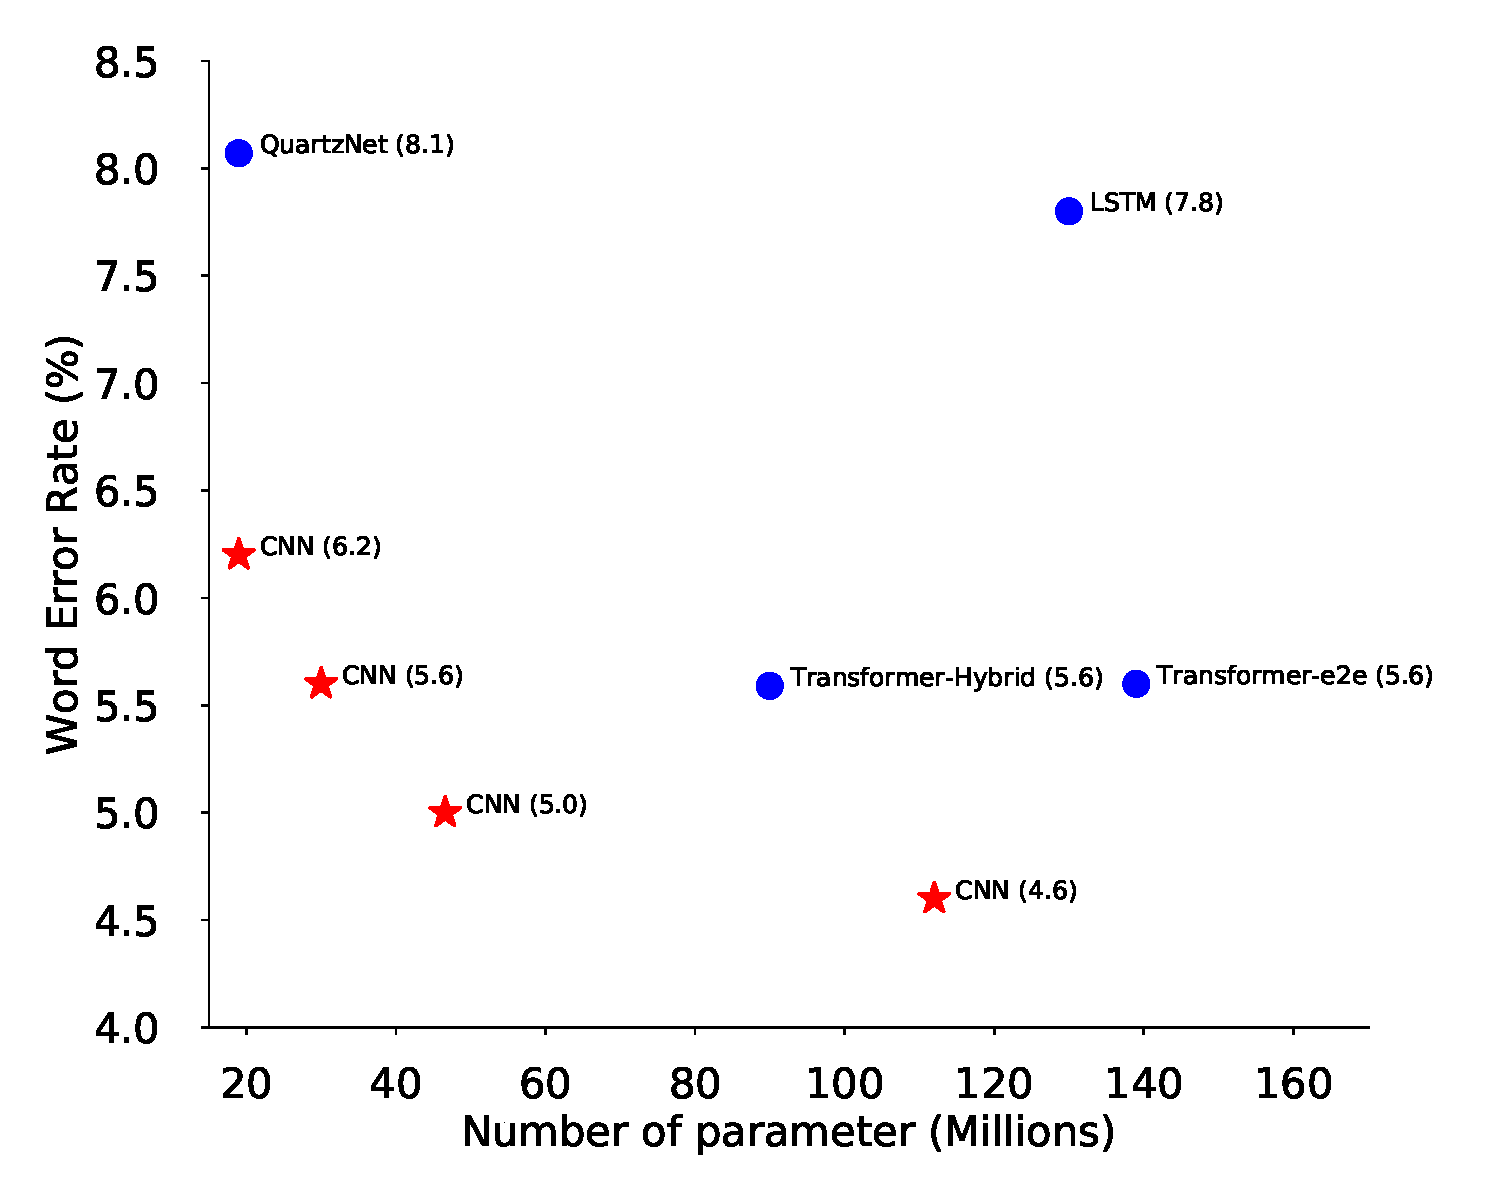
\includegraphics[width=1\columnwidth]{figure/plot_1}
\par\end{centering}
\caption{LibRispeech Testother WER v.s. Model parameters}
\end{figure}

\subsection{Result on LibriSpeech}
Table \ref{tab:libri_speech_main} showed the result of our model on LibriSpeech test-clean/test-other against a few state-of-the-art methods include: transformer transducer, Jasper, QuartzNet and XXX.

Without language model, the performance of our model already surpassed the best known CNN model even with external language model. With the language model added, our model achieves the lowest word error rate among all the existing models. This clearly demonstrated the effectiveness of our model.

\begin{table}
\begin{centering}
\begin{tabular}{c|c|cc|cc}
\hline 
\multirow{2}{*}[-0.5em]{Model} & \multirow{2}{*}[-0.5em]{\#Params(M)} & \multicolumn{2}{c|}{Without LM} & \multicolumn{2}{c}{With LM}\\ \cline{3-6}
& & \makecell{test\\ clean} & \makecell{test\\ other} & \makecell{test \\clean} & \makecell{test \\ other}\\
\hline 
\hline 
QuartzNet~\cite{kriman2019quartznet}& 19 &3.90 & 11.28 & 2.69 & 7.25\tabularnewline
Hybrid~\cite{wang2019transformer}& - & - & - & 2.26 & 4.85\tabularnewline
Transformer~\cite{zhang2020transformer} & 139 & 2.4 & 5.6 & 2.0 & 4.6\tabularnewline
Ours & 30 & \textbf{2.4} & \textbf{5.4} &  & \tabularnewline
Ours & 46 & \textbf{2.3} & \textbf{5.0} &  & \tabularnewline
Ours & 112 & \textbf{2.1} & \textbf{4.6} & \textbf{2.0} & \textbf{4.1}
\\\hline
\hline 
\end{tabular}
\par\end{centering}
\caption{Comparison of our model against other existing models. Our model achieves superior performance both with and without language models.}
\label{tab:libri_speech_main}
\end{table}

% Table 1: With SE, without SE, SE with window size (a few?)

\subsection{Effect of context size}
To validate the effectiveness of adding global context in the CNN model for speech, we performed an ablation study on how the squeeze-and-excitation module affects the WER on LibriSpeech test-clean/test-other. The original model with all squeeze-and-excitation modules removed serves as the baseline to compare with the original model. 
Note that the squeeze-and-excitation module uses the whole utterance as the context; it has the maximal temporal length of context. This motivates us to study how the temporal length of the context impacts the model performance. To reduce the context to a window smaller than the whole utterance, we replace the global average pooling operator of the squeeze-and-excitation module by a convolutional averaging operator with a kernel size that corresponds to the context window; we apply the same fully connected layers on each context vector, and impose it on the feature of each time step. In this study, we tried window size of $100$ and $200$. 

Table~\ref{tab:context_size} illustrated the result.
% Performed on top of a standard model
% Table 2

\begin{table}
\begin{centering}
\begin{tabular}{c|cc}
\hline 
Context & \makecell{test\\ clean} & \makecell{test\\ other} \\
\hline 
\hline 
None & ? & ? \tabularnewline
256 & ? & ? \tabularnewline
512 & 2.4 & 5.2\tabularnewline
1024 & 2.3 & 5.1\tabularnewline
global & \textbf{2.3} & \textbf{4.9}\\\hline
\hline 
\end{tabular}
\par\end{centering}
\caption{Ablation study on the temporal length of the context. }
\label{tab:libri_speech_main}
\end{table}


\subsection{Depth, width, filter size and downsampling}
\textit{Depth\ \ } We can increase the model capacity by adding extra convolutional blocks that maintains the number of channels of the encoded features. This also introduces additional computations. We perform a sweeping on the number of extra convolutional layers of the baseline model, and summary the WERs on LibriSpeech test-clean/test-other in Table \ref{tab:ablation_depth}. From the table, we can clearly see the reduction on WER due to the extra capacity of the network, until when the number of layers reach $XX$ and the model saturates.
\begin{table}
\begin{centering}
\begin{tabular}{c|cc}
\hline 
\# Extra Layers & \makecell{test\\ clean} & \makecell{test\\ other} \\
\hline 
\hline 
0 & ? & ? \tabularnewline
15 & ? & ? \tabularnewline
512 & ? & ?\tabularnewline
1024 & ? & ?\tabularnewline
\hline 
\end{tabular}
\par\end{centering}
\caption{Ablation study on the depth of the network.}
\label{tab:ablation_depth}
\end{table}


\vspace{0.1in}
\noindent \textit{Width\ \ }

\begin{table}
\begin{centering}
\begin{tabular}{c|ccc}
\hline 
$\alpha$ & \#Params(M) & \makecell{test\\ clean} & \makecell{test\\ other} \\
\hline 
\hline 
1.25 & 46 & 2.3 & 4.9 \tabularnewline
1.5 & 46 & 2.2 & 4.8 \tabularnewline
1.75 & 87 & 2.2 & 4.7\tabularnewline
2 & 112 & 2.2 & 4.6\tabularnewline
\hline 
\end{tabular}
\par\end{centering}
\caption{Ablation study on the width of the network.}
\label{tab:ablation_depth}
\end{table}

We also scale the width of the network (i.e., the number of channels) and sees how it impacts the model performance. Specifically, we take the baseline model and scale up the output number of channels of all the convolutional kernels by $\alpha, \alpha > 1$. \zhengdong{What would be the observation?}

\vspace{0.1in}
\noindent
\textit{Downsampling and filter size\ \ }
Table \ref{tab:ablation_downsampling} summarizes the flops and WER on LibriSpeech with and without progressive downsampling. For the reference model with no progressive downsampling, we use the same CNN architectur from the QuartzNet, whose filter size ranges from $11$ to $70$\zhengdong{Confirm}. For the model with progressive downsampling, we sweep the filter size in $\{5, 11, 21\}$. Table \ref{tab:ablation_downsampling} suggests that progressive downsampling introduces significant saving in the number of flops. Moreover, it actually benefits the accuracy of the model slightly. In addition, with progressive downsampling, increasing the filter size hurts the model. This suggests model overfitting.

To qualitatively understand this phenomenon, we plot the initial receptive field of each of the models at each encoder output time step using the technique from \cite{luo2016understanding}. Figure ~\ref{fig:effective_receptive_field} plots the result. Clearly we can see that an encoder output of the QuartzNet architecture effecitvely covers the entire utterance spanning tens of seconds. Our network is much more modest, but still covers a few seconds of an audio sequence to extract rich enough information.

\subsection{Large scale dataset}
Finally, we show that the proposed architecture is also effective on large scale datasets. We use a experimental setup similar to \cite{Chiu19longform}, where the training set has 200K hours of public Youtube videos with semi-supervised transcripts generated by the approach in \cite{hank}. We evaluate on two test sets: \textit{Yt-long } of 87 videos with a total of 24.12 hours and \textit{Yt-short} of 119 videos with a total duration of 24.12 hours. Both sets come with diverse and challenging acoustic environments.

% Preview source code for paragraph 0

\begin{table}
\begin{centering}
\begin{tabular}{cccc}
\hline 
Model & \#Params (M) & YT-short & YT-long\tabularnewline
\hline 
\hline 
LSTM & 192 & 9.1 & 14.8\tabularnewline
CNN & 112 & 9.0 & 14.6\tabularnewline
CNN & 178 & 8.4 & 14.4\tabularnewline
\hline 
\end{tabular}
\par\end{centering}
\caption{Comparison with previous best results on Youtube test sets}

\end{table}


